\documentclass[10pt]{beamer}
\mode<presentation>
\usepackage{beamerthemesplit}
\usepackage{graphicx}
\usepackage{booktabs}
\usepackage{amsmath}
\usepackage{textpos}
\usepackage{pgfplots}
\usepackage{tikz}
\usepackage{hyperref}
\usepackage{caption}
\usepackage{listings}


% import citation package
\usepackage{biblatex}
\addbibresource{presentation.bib}
\AtBeginBibliography{\small}

\usetikzlibrary{shapes.geometric, arrows}
\usetikzlibrary {datavisualization} 
\pgfplotsset{compat=1.18, width = 7cm}
\usetikzlibrary{patterns}
\usetheme{Ilmenau} % AnnArbor, Ilmenau, Darmstadt, Dresden, CambridgeUS, Frankfurt, Singapore
\newtheorem{dn}{Định nghĩa}[section]
\newtheorem{dl}{Định lý}[section]
\newtheorem{tc}{Tính chất}[section]
\newtheorem{hq}{Hệ quả}[section]
\newtheorem{bd}{Bổ đề}[section]
\newtheorem{md}{Mệnh đề}[section]
\newtheorem{vd}{Ví dụ}[section]
\newtheorem{nx}{Nhận xét}[section]
\newtheorem{cy}{Chú ý}[section]
\newcommand{\dom}{\text{{\rm dom}}}
\newcommand{\epi}{\text{{\rm epi}}}
\newcommand{\Min}{\text{{\rm Min}}}
\setbeamertemplate{theorems}[numbered]
\setbeamertemplate{definitions}[numbered]
\setbeamertemplate{footline}[frame number]
\usepackage{algorithm}
\usepackage{color}
\usepackage{algorithmic}
\usepackage{footmisc}
\usepackage{indentfirst} 
\usepackage{comment}
\AtBeginEnvironment{proof}{%
  \setbeamercolor{block title}{use=example text,fg=white,bg=example text.fg!75!black}
  \setbeamercolor{block body}{parent=normal text,use=block title example,bg=block title example.bg!10!bg}
}
\renewcommand{\thefootnote}{\arabic{footnote}}
\usefonttheme{professionalfonts}
\setbeamercolor{normal text}{bg=white,fg=black}
\renewcommand{\thefootnote}{\arabic{footnote}}
\beamertemplatetransparentcoveredhigh
\usetheme[progressbar=frametitle]{metropolis}
\usepackage{appendixnumberbeamer}

\usepackage[utf8]{vietnam}

\usepackage{booktabs}
\usepackage[scale=2]{ccicons}

\usepackage{pgfplots}
\usepgfplotslibrary{dateplot}

\usepackage{xspace}
\newcommand{\themename}{\textbf{\textsc{metropolis}}\xspace}
\definecolor{mSybilaRed}{HTML}{990000}

\setbeamercolor{title separator}{
  fg=mSybilaRed
}

\setbeamercolor{progress bar}{%
  fg=mSybilaRed,
  bg=mSybilaRed!90!black!30
}

\setbeamercolor{progress bar in section page}{
  use=progress bar,
  parent=progress bar
}

\setbeamercolor{alerted text}{%
  fg=mSybilaRed
}

\setbeamertemplate{footline}
{
  \leavevmode
  \hbox{
  \begin{beamercolorbox}[wd=.15\paperwidth,ht=2.25ex,dp=1ex,center]{title in head/foot}
  \end{beamercolorbox}

  \begin{beamercolorbox}[wd=.7\paperwidth,ht=2.25ex,dp=1ex,center]{author in head/foot}
    \usebeamerfont{author in head/foot}\insertshorttitle
  \end{beamercolorbox}

  \begin{beamercolorbox}[wd=.15\paperwidth,ht=2.25ex,dp=1ex,center]{title in head/foot}
    \insertframenumber{} / \inserttotalframenumber
  \end{beamercolorbox}
  }
}

\title{Chạy số liệu minh hoạ bằng thư viện TiLearn}


\titlegraphic{\hfill 
\includegraphics[height=1cm]{tilearn.png}}
%\titlegraphic{\hfill
\includegraphics[height=0.6cm]{sybila-logo/new.png}}
%\titlegraphic{\hfill
\includegraphics[height=0.6cm]{sybila-logo/old.png}}
%\titlegraphic{\hfill
\includegraphics[height=0.6cm]{sybila-logo/old-flat.png}}

\date{\today}
\author{Hướng dẫn: TS. Lê Minh Huy}
% \institute{Sinh viên lớp: DTU1221, Khóa: 22 @ Trường Đại học Sài Gòn}

%\title{Metropolis}
\subtitle{Thực hiện: Nguyễn Chí Bằng}
% \date{\today}
%\date{}
%\author{Matthias Vogelgesang}
%\institute{Center for modern beamer themes}
%\titlegraphic{\hfill
\includegraphics[height=1.5cm]{logo.pdf}}

\definecolor{codegreen}{rgb}{0,0.6,0}
\definecolor{codegray}{rgb}{0.5,0.5,0.5}
\definecolor{codepurple}{rgb}{0.58,0,0.82}
\definecolor{backcolour}{rgb}{0.95,0.95,0.92}

\lstdefinestyle{mystyle}{
    backgroundcolor=\color{backcolour},   
    commentstyle=\color{codegreen},
    keywordstyle=\color{magenta},
    numberstyle=\tiny\color{codegray},
    stringstyle=\color{codepurple},
    basicstyle=\ttfamily\footnotesize,
    breakatwhitespace=false,         
    breaklines=true,                 
    captionpos=b,                    
    keepspaces=true,                 
    numbers=left,                    
    numbersep=5pt,                  
    showspaces=false,                
    showstringspaces=false,
    showtabs=false,                  
    tabsize=2
}

\lstset{style=mystyle}

\begin{document}

\begin{frame}
  \titlepage
\end{frame}

\begin{frame}
    \frametitle{NỘI DUNG}
    \tableofcontents
\end{frame}

\section{Giới thiệu về thư viện}

\begin{frame}{Giới thiệu về thư viện TiLearn}
\textbf{TiLearn} là sự kết hợp của Time và Machine Learning (học máy), thư viện được xây dựng với mục đích ban đầu hướng đến mục tiêu tự động hoá quá trình đánh giá trọng số cho công việc ($w_j$) và cải thiện quá trình phân nhánh (Learning to Branch) bằng phương pháp học máy.

\begin{figure}[h]
\centering
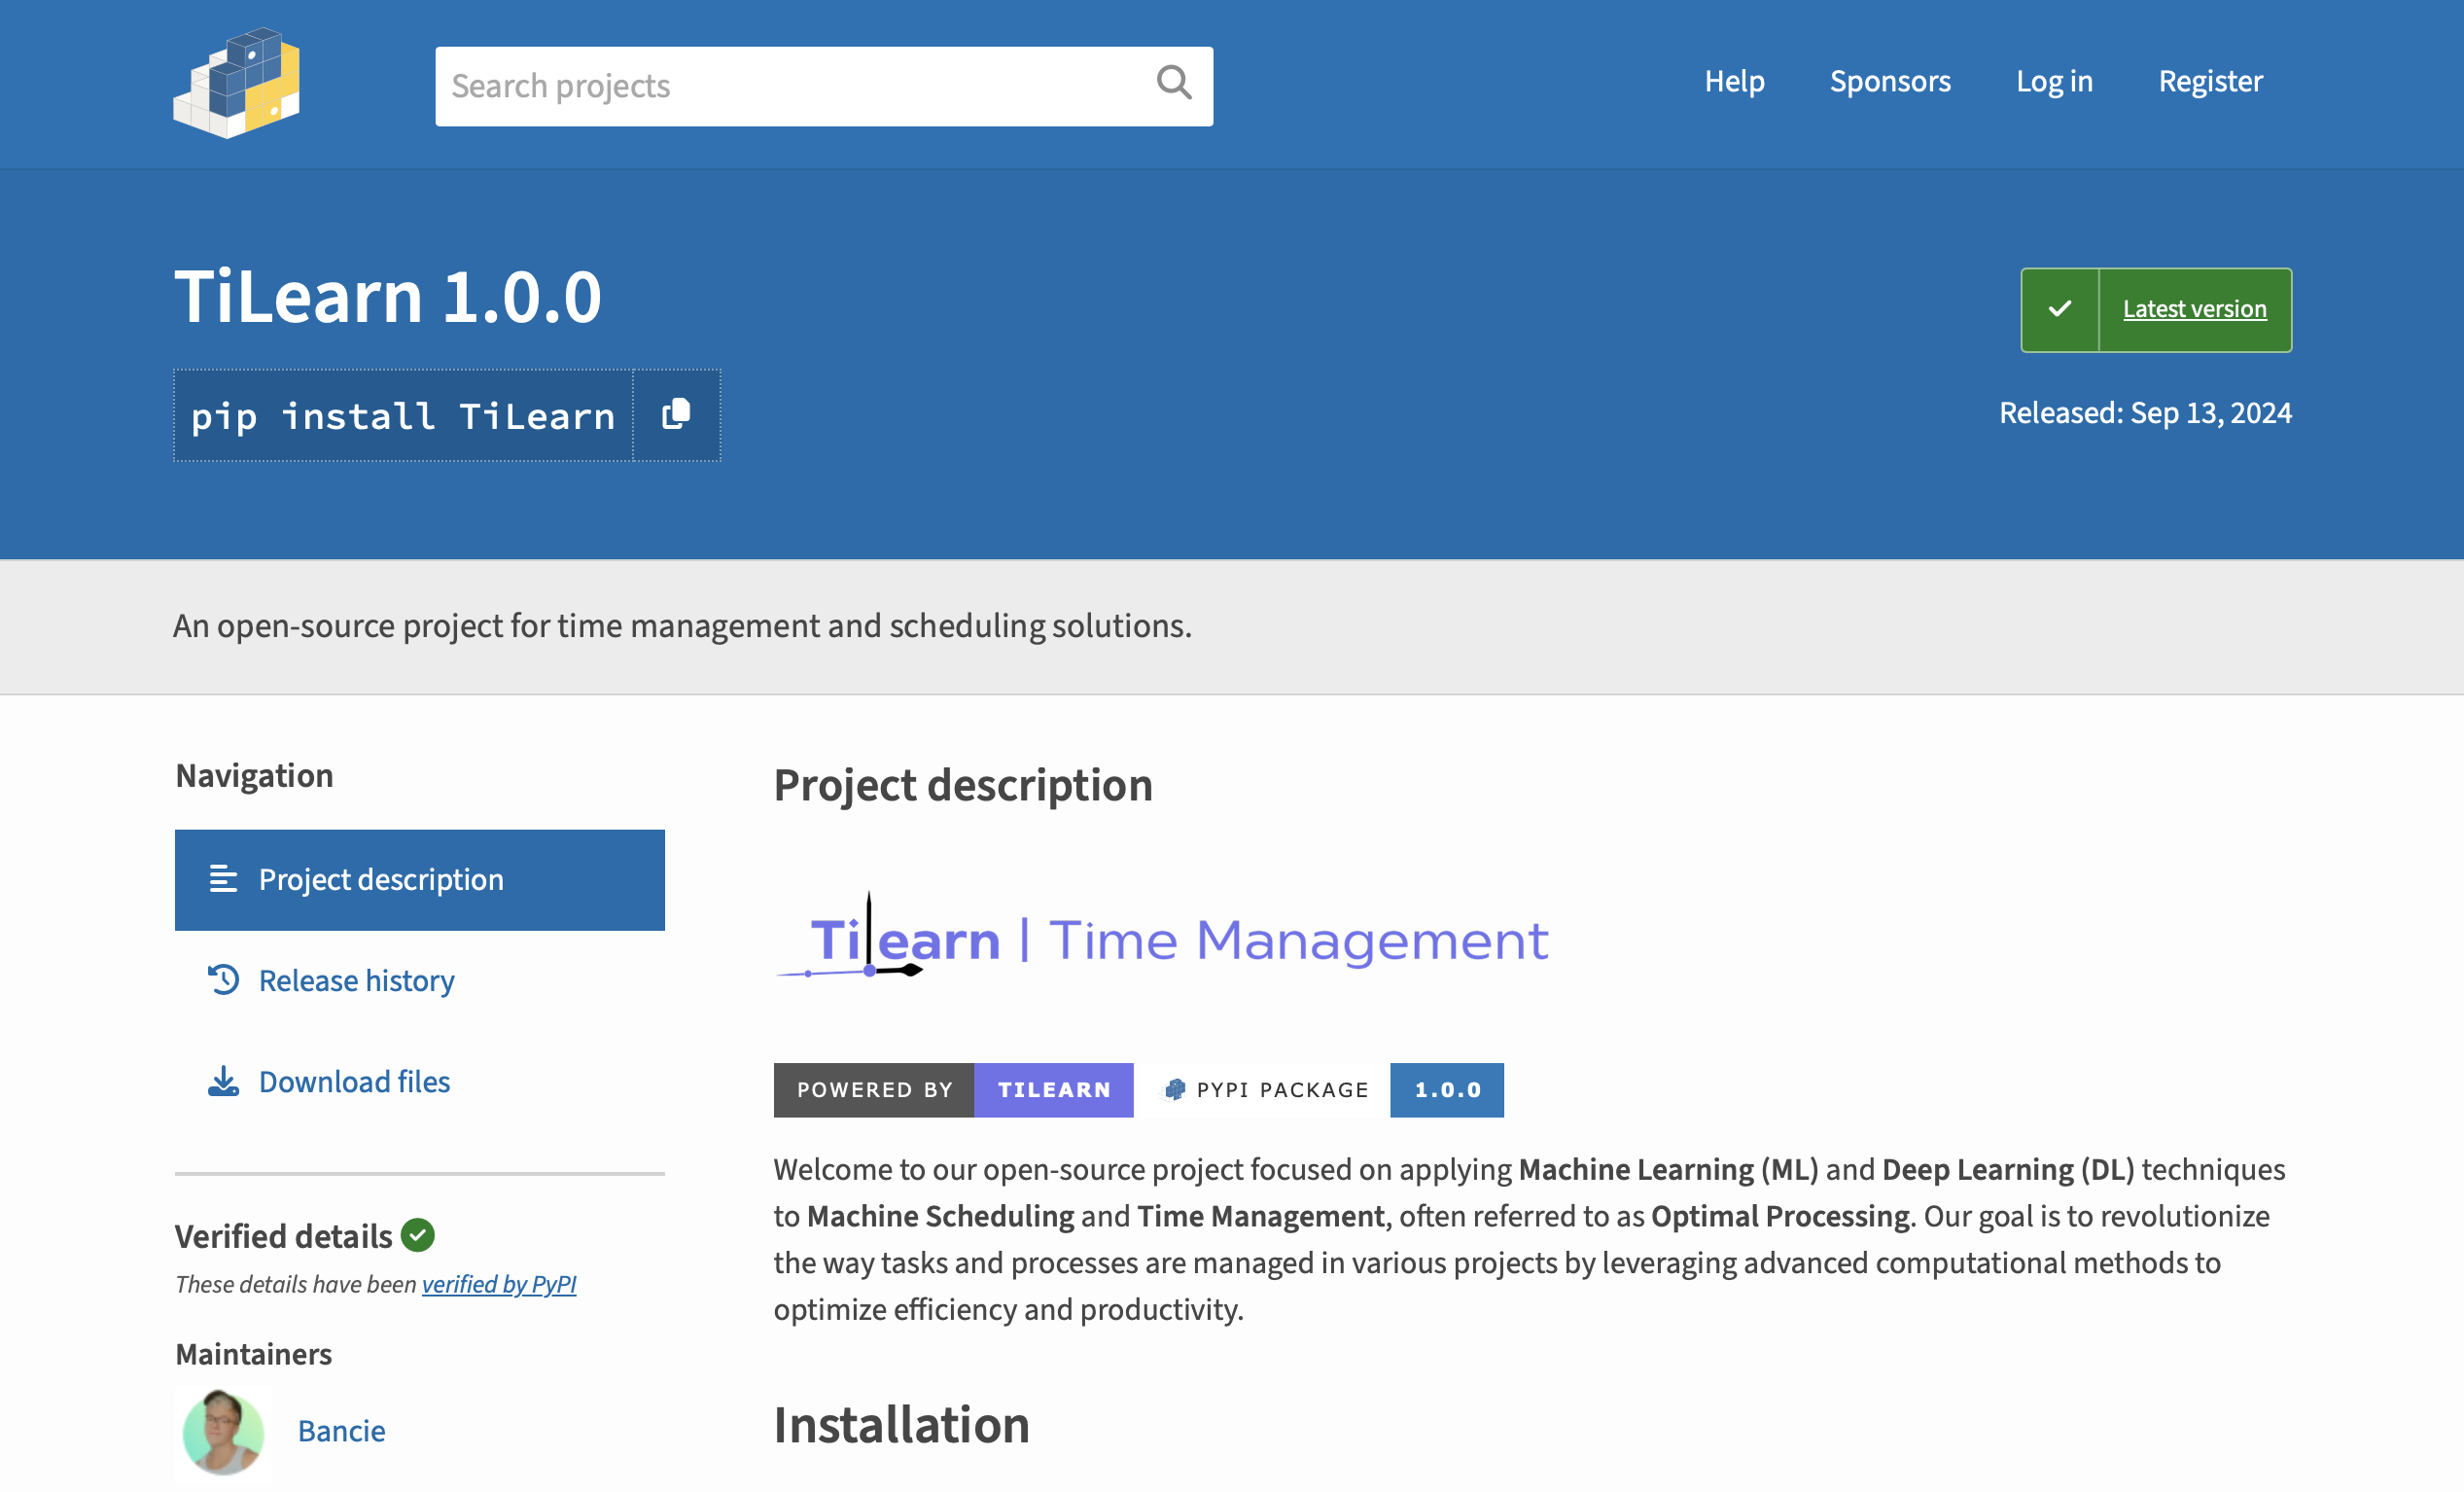
\includegraphics[width=0.5\linewidth]{pypi_capture.png}
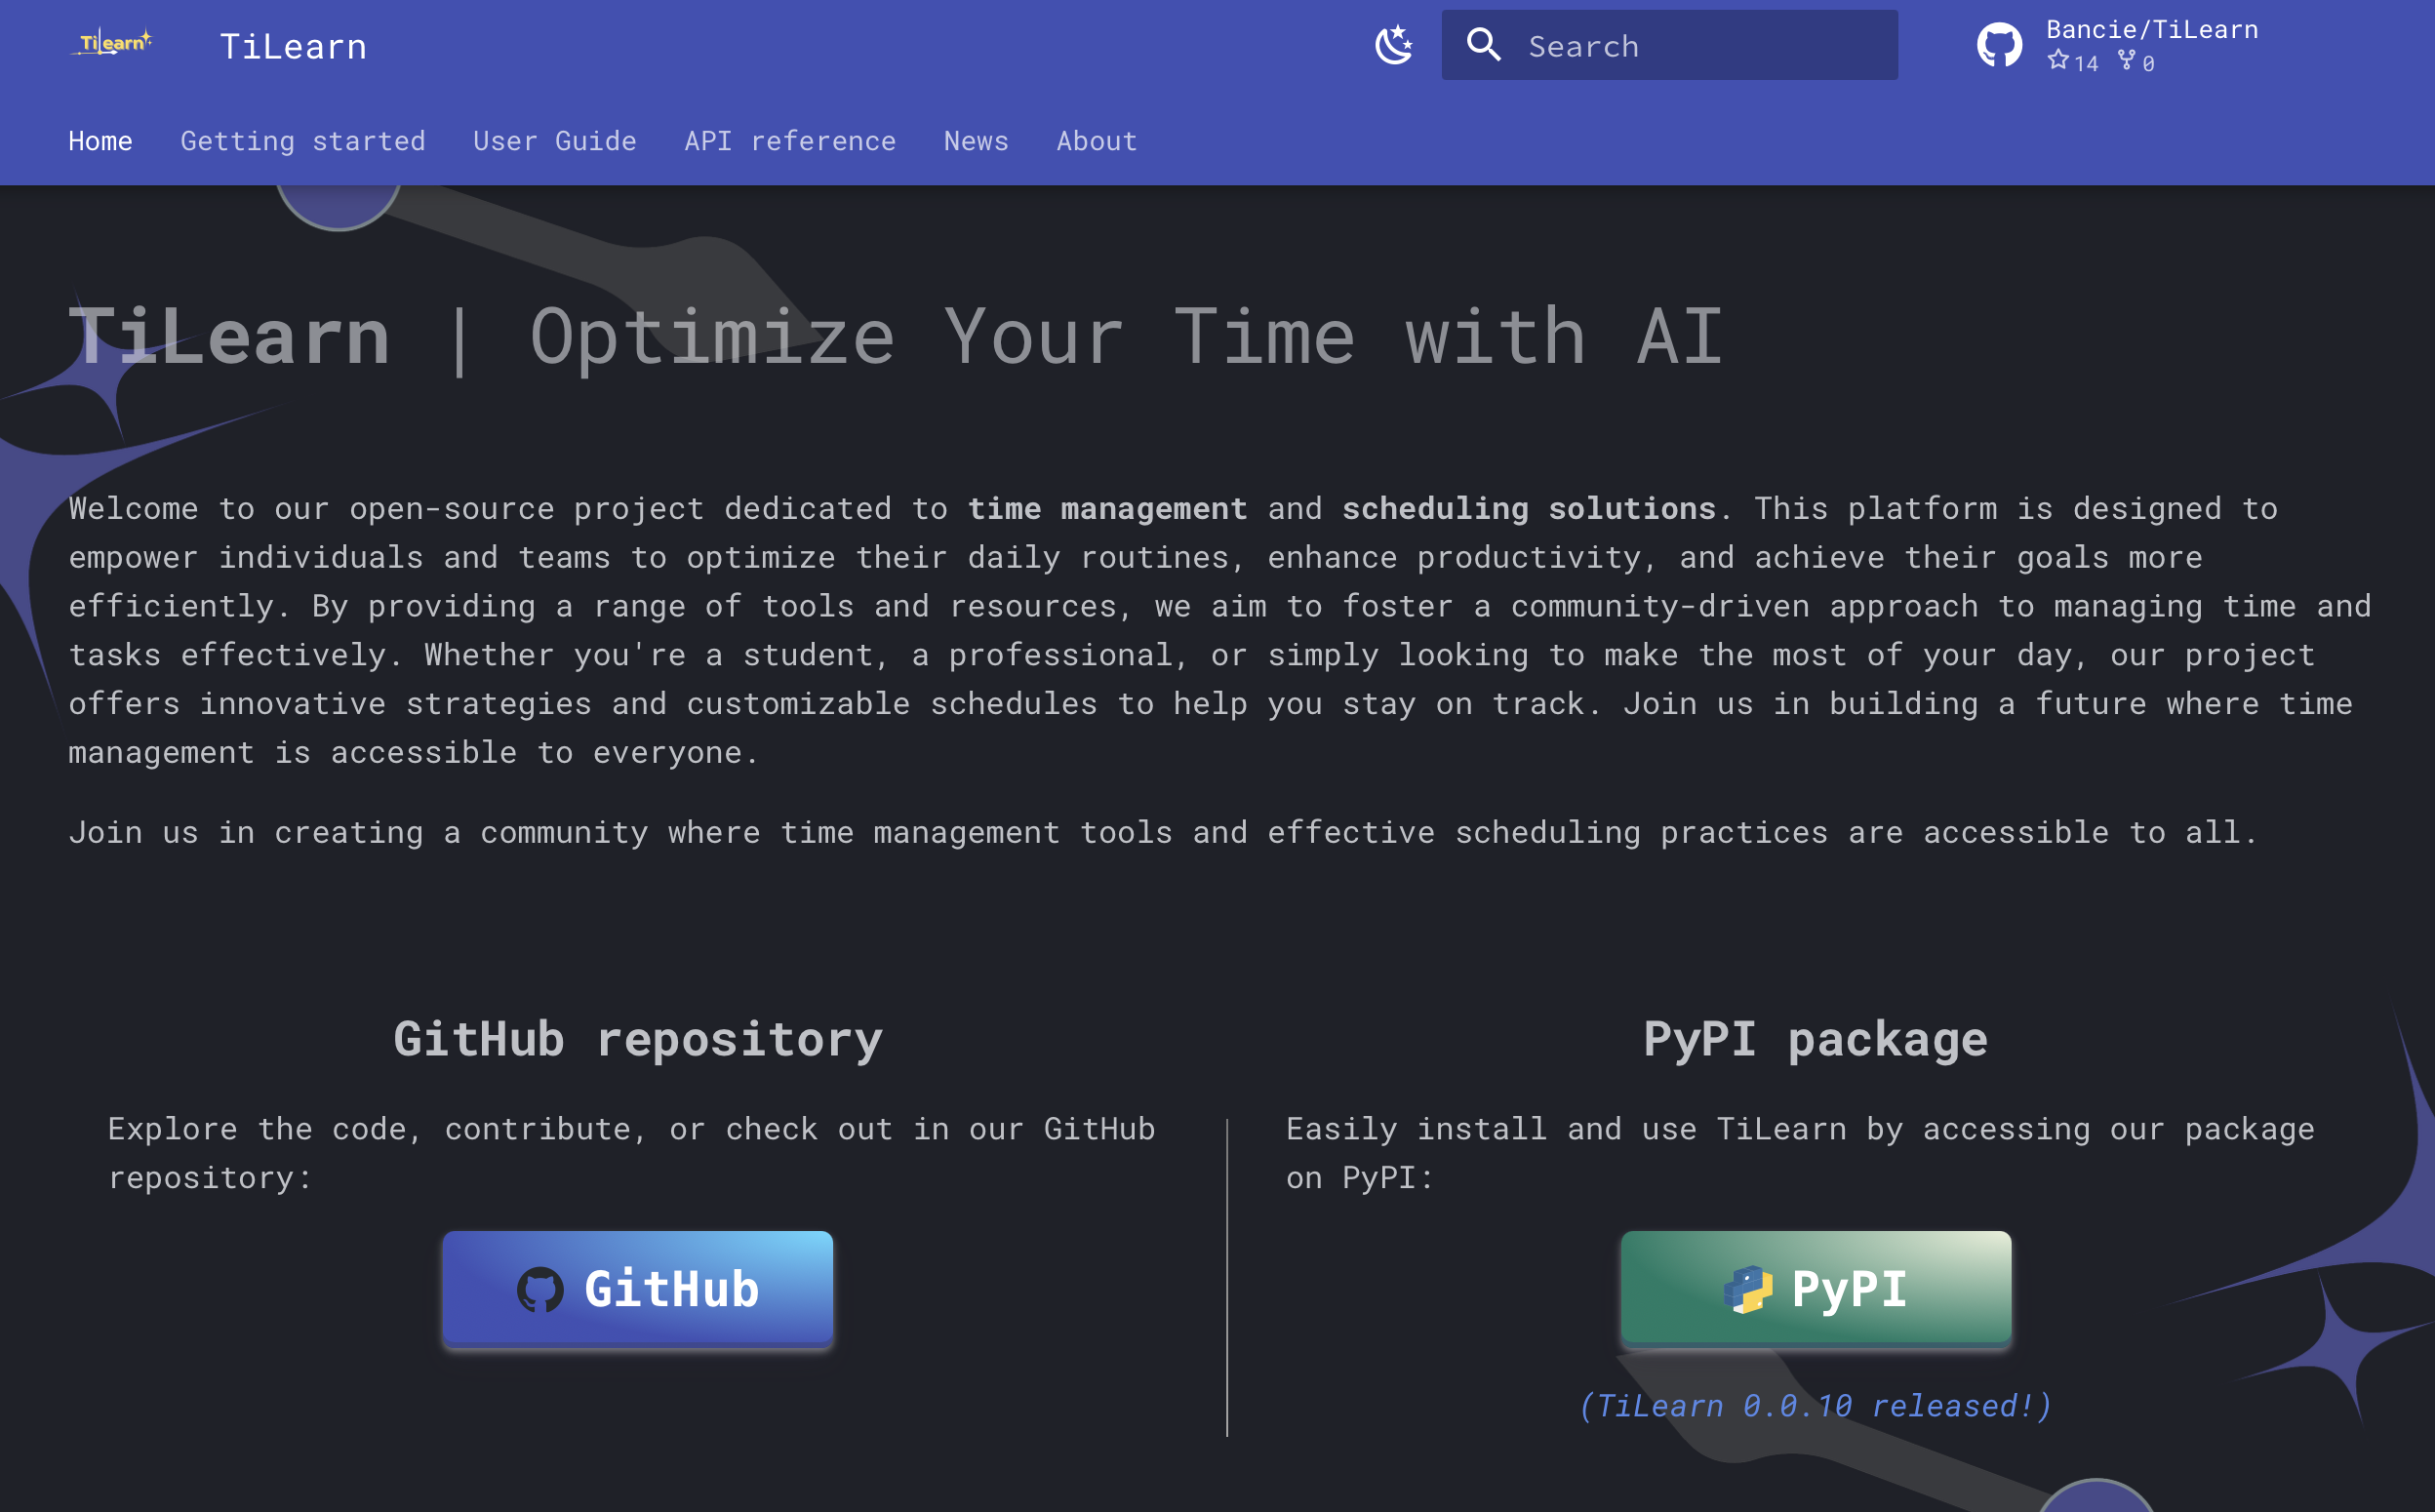
\includegraphics[width=0.489\linewidth]{web_capture.png}
\end{figure}
\end{frame}

\begin{frame}{Giới thiệu về thư viện TiLearn}
Mã nguồn hiện đã được tải lên \textbf{GitHub}, quét mã bên dưới để truy cập:

\begin{figure}[h]
\centering

\includegraphics[width=0.4\linewidth]{tilearn_github.png}
\caption{Mã nguồn GitHub.}
\end{figure}
\end{frame}


\begin{frame}{Giới thiệu về thư viện TiLearn}
Thư viện cũng đã được công bố trên trang \textbf{PyPI} giúp dễ dàng tải và sử dụng, quét mã bên dưới để truy cập:

\begin{figure}[h]
\centering

\includegraphics[width=0.4\linewidth]{tilearn_pypi.png}
\caption{Trang thư viện PyPI.}
\end{figure}
\end{frame}

\begin{frame}{Giới thiệu về thư viện TiLearn}
Bên cạnh đó, \textbf{web document} cũng được tạo để cung cấp tài liệu hướng dẫn cách sử dụng, cách chạy cũng như cách thư viện hoạt động, quét mã bên dưới để truy cập:

\begin{figure}[h]
\centering

\includegraphics[width=0.4\linewidth]{tilearn_docs.png}
\caption{Web document.}
\end{figure}
\end{frame}

\begin{frame}{Giới thiệu về thư viện TiLearn}
    Hiện thư viện đã hoàn thiện các tính năng sau:
    \begin{itemize}
    \item Hàm chạy thuật toán EDD.
    \medskip
    \item Hàm chạy thuật toán WSPT.
    \medskip
    \item Hàm giúp xử lý bài toán $1||\sum C_j$.
    \medskip
    \item Hàm giúp xử lý bài toán $1||\sum w_j C_j$.
    \medskip
    \item Hàm giúp xử lý bài toán $1|prec|\sum C_j$.
    \medskip
    \item Hàm giúp xử lý bài toán $1|prec|\sum w_j C_j$.
    \medskip
    \item Hàm giúp xử lý hỗn hợp 2 bài toán $1|prec|\sum w_j C_j$ và $1||\sum w_j C_j$.
    \end{itemize}
\end{frame}



\begin{frame}[fragile]{Giới thiệu về thư viện TiLearn}
\begin{itemize}
\item<1-> Để sử dụng thư viện, ta tải thư viện bằng lệnh sau:
\medskip
\begin{lstlisting}
    pip install tilearn
\end{lstlisting}
\medskip
% Một số thư viện hỗ trợ phân tích dữ liệu:
% \begin{lstlisting}
%     pip install pandas
%     pip install ipython
%     pip install jinja2
% \end{lstlisting}
\item<2-> Thực hiện khai báo thư viện như sau:
\medskip
\begin{lstlisting}[language=Python]
    import tilearn as tl
    from tilearn import _plat as pl
\end{lstlisting}
\end{itemize}

\end{frame}

% \begin{frame}[fragile]{Giới thiệu về thư viện TiLearn}


% Thư viện hỗ trợ phân tích dữ liệu:
% \medskip
% \begin{lstlisting}[language=Python]
%     import csv
%     import pandas as pd
%     from IPython.display import display
%     import matplotlib.pyplot as plt
% \end{lstlisting}

% \end{frame}


\section{Chạy số liệu minh hoạ}

\begin{frame}{Chạy số liệu minh hoạ}
Giả sử ta cần xử lý 3 danh sách công việc sau:
\begin{columns}
    \begin{column}{0.5\textwidth}
    \begin{table}[t]
        \centering
        \resizebox{85pt}{!}{%
            \begin{tabular}{|l|c|c|c|c|}
            \hline
            \textbf{Name} & \textbf{p} & \textbf{r} & \textbf{d} & \textbf{w} \\
            \hline
            Job 1  & 4  & 0  & 100 & 0.65 \\
            Job 2  & 1  & 0  & 100 & 0.84 \\
            Job 3  & 3  & 0  & 100 & 0.46 \\
            Job 4  & 3  & 0  & 100 & 0.79 \\
            Job 5  & 1  & 0  & 100 & 0.17 \\
            Job 6  & 3  & 0  & 100 & 0.50 \\
            Job 7  & 4  & 0  & 100 & 0.95 \\
            Job 8  & 2  & 0  & 100 & 0.14 \\
            Job 9  & 5  & 0  & 100 & 0.52 \\
            Job 10 & 2  & 0  & 100 & 0.40 \\
            Job 11 & 4  & 0  & 100 & 0.55 \\
            Job 12 & 1  & 0  & 100 & 0.39 \\
            Job 13 & 2  & 0  & 100 & 0.57 \\
            Job 14 & 1  & 0  & 100 & 0.90 \\
            Job 15 & 1  & 0  & 100 & 0.22 \\
            \hline
            \end{tabular}%
        }
        \caption{Danh sách 1.}
        \label{tab:job_table}
    \end{table}
\end{column}
\begin{column}{0.5\textwidth}
    Trong đó, danh sách 1 các công việc độc lập và \textbf{không tồn tại} ràng buộc thứ tự, tức thuộc dạng bài toán $1||\sum w_j C_j$.
\end{column}
\end{columns}

\end{frame}

\begin{frame}{Chạy số liệu minh hoạ}
\begin{columns}
\begin{column}{0.5\textwidth}
    \begin{table}[ht]
        \centering
        \resizebox{160pt}{!}{%
            \begin{tabular}{|l|c|c|c|c|}
            \hline
            \textbf{Name} & \textbf{p} & \textbf{r} & \textbf{d} & \textbf{w} \\
            \hline
            Job 16 & 4  & 0  & 100 & 0.70 \\
            Job 17 & 3  & 0  & 100 & 0.95 \\
            Job 18 & 4  & 0  & 100 & 0.49 \\
            Job 19 & 1  & 0  & 100 & 0.13 \\
            Job 20 & 5  & 0  & 100 & 0.94 \\
            Job 21 & 1  & 0  & 100 & 0.57 \\
            Job 22 & 4  & 0  & 100 & 0.79 \\
            \hline
            \end{tabular}%
        }
        \caption{Danh sách 2.}
        \label{tab:extended_job_table}
    \end{table}
\end{column}
\begin{column}{0.5\textwidth}
Trong đó, danh sách 2 \textbf{tồn tại} ràng buộc thứ tự, tức thuộc dạng bài toán $1|prec|\sum w_j C_j$.
\end{column}
\end{columns}
\end{frame}

\begin{frame}{Chạy số liệu minh hoạ}
\begin{columns}
\begin{column}{0.5\textwidth}
    \begin{table}[ht]
        \centering
        \resizebox{150pt}{!}{%
            \begin{tabular}{|l|c|c|c|c|}
            \hline
            \textbf{Name} & \textbf{p} & \textbf{r} & \textbf{d} & \textbf{w} \\
            \hline
            Job 23 & 4  & 0  & 100 & 0.24 \\
            Job 24 & 1  & 0  & 100 & 0.54 \\
            Job 25 & 2  & 0  & 100 & 0.81 \\
            Job 26 & 2  & 0  & 100 & 0.41 \\
            Job 27 & 5  & 0  & 100 & 0.22 \\
            Job 28 & 2  & 0  & 100 & 0.29 \\
            Job 29 & 5  & 0  & 100 & 0.65 \\
            Job 30 & 4  & 0  & 100 & 0.69 \\
            \hline
            \end{tabular}%
        }
        \caption{Danh sách 3.}
        \label{tab:further_extended_job_table}
    \end{table}
\end{column}
\begin{column}{0.5\textwidth}
Tương tự, danh sách 3 \textbf{tồn tại} ràng buộc thứ tự, tức thuộc dạng bài toán $1|prec|\sum w_j C_j$.
\end{column}
\end{columns}
\end{frame}

\begin{frame}{Chạy số liệu minh hoạ}
Cấu trúc tập tin được thiết lập như sau:
\medskip
\begin{figure}[h]
\centering
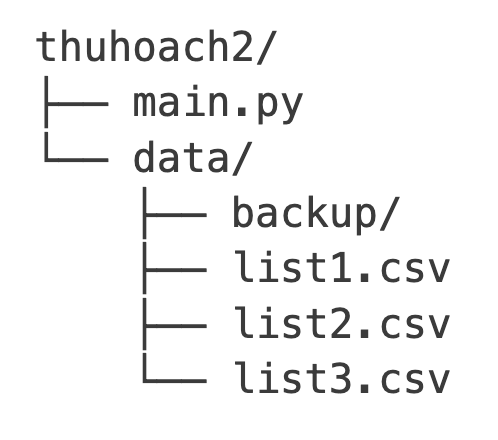
\includegraphics[width=0.4\linewidth]{path.png}
\caption{Cấu trúc tập tin.}
\end{figure}
\end{frame}

\begin{frame}[fragile]{Chạy số liệu minh hoạ}
\onslide<1->{Ta thực hiện hai báo đường dẫn dữ liệu như sau:}
\begin{lstlisting}[language=Python]
    original = 'thuhoach2/data'
    backup = 'thuhoach2/data/backup'
    list1 = 'thuhoach2/data/list1.csv'
    list2 = 'thuhoach2/data/list2.csv'
    list3 = 'thuhoach2/data/list3.csv'
\end{lstlisting}
\onslide<2->{Tiếp theo, ta chọn dạng bài toán cho từng danh sách bằng cách thiết lập tham số \textbf{prec} như sau:}
    
\begin{itemize}
\item<2-> \textbf{prec=0} cho bài toán không tồn tại ràng buộc thứ tự.
\item<2-> \textbf{prec=1} cho bài toán tồn tại ràng buộc thứ tự.

\begin{lstlisting}[language=Python]
    lists = [
        pl.List(file_path=list1, prec=0),
        pl.List(file_path=list2, prec=1),
        pl.List(file_path=list3, prec=1),
    ]
\end{lstlisting}
\end{itemize}

\end{frame}

\begin{frame}[fragile]{Chạy số liệu minh hoạ}
\onslide<1->{Ta chạy chương trình bằng lệnh sau:}
\begin{lstlisting}[language=Python]
    schedule = tl.optimal_list(lists, original, backup)
    print(schedule)
\end{lstlisting}

\onslide<2->{{\scriptsize [['Job 14', 1.0, 0, 100, 0.9, 0.9], ['Job 2', 1.0, 0, 100, 0.84, 0.84], ['Job 12', 1.0, 0, 100, 0.39, 0.39], ['Job 13', 2.0, 0, 100, 0.57, 0.285], ['Job 4', 3.0, 0, 100, 0.79, 0.26333333333333336], ['Job 7', 4.0, 0, 100, 0.95, 0.2375], ['Job 16', 4.0, 0, 100, 0.7, 0.175], ['Job 17', 3.0, 0, 100, 0.95, 0.2357142857142857], ['Job 23', 4.0, 0, 100, 0.24, 0.06], ['Job 24', 1.0, 0, 100, 0.54, 0.156], ['Job 25', 2.0, 0, 100, 0.81, 0.22714285714285715], ['Job 15', 1.0, 0, 100, 0.22, 0.22], ['Job 26', 2.0, 0, 100, 0.41, 0.205], ['Job 10', 2.0, 0, 100, 0.4, 0.2], ['Job 18', 4.0, 0, 100, 0.49, 0.1225], ['Job 19', 1.0, 0, 100, 0.13, 0.124], ['Job 20', 5.0, 0, 100, 0.94, 0.156], ['Job 21', 1.0, 0, 100, 0.57, 0.19363636363636363], ['Job 5', 1.0, 0, 100, 0.17, 0.17], ['Job 6', 3.0, 0, 100, 0.5, 0.16666666666666666], ['Job 1', 4.0, 0, 100, 0.65, 0.1625], ['Job 3', 3.0, 0, 100, 0.46, 0.15333333333333335], ['Job 11', 4.0, 0, 100, 0.55, 0.1375], ['Job 22', 4.0, 0, 100, 0.47, 0.1175], ['Job 27', 5.0, 0, 100, 0.22, 0.044], ['Job 28', 2.0, 0, 100, 0.29, 0.07285714285714286], ['Job 29', 5.0, 0, 100, 0.65, 0.09666666666666668], ['Job 30', 4.0, 0, 100, 0.69, 0.115625], ['Job 9', 5.0, 0, 100, 0.52, 0.10400000000000001], ['Job 8', 2.0, 0, 100, 0.14, 0.07]]}}

\end{frame}
\section*{Dữ liệu trực quan}

\begin{frame}{Dữ liệu trực quan}
\begin{figure}[h]
\centering
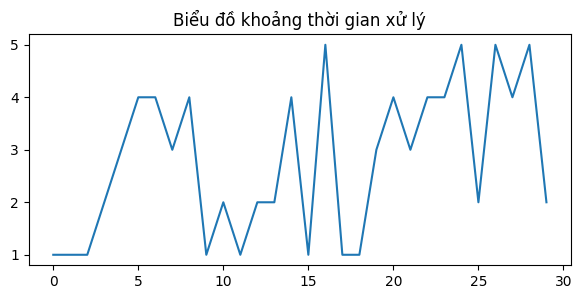
\includegraphics[width=0.7\linewidth]{output_p.png}
\caption{Biểu đồ khoảng thời gian xử lý.}
\end{figure}

Dựa vào biểu đồ trên, có thể thấy rằng sau khi tối ưu hóa danh sách công việc, thời gian xử lý của từng công việc có \textbf{xu hướng tăng} từ công việc đầu tiên đến công việc cuối cùng.
\end{frame}

\begin{frame}{Dữ liệu trực quan}
\begin{figure}[h]
\centering
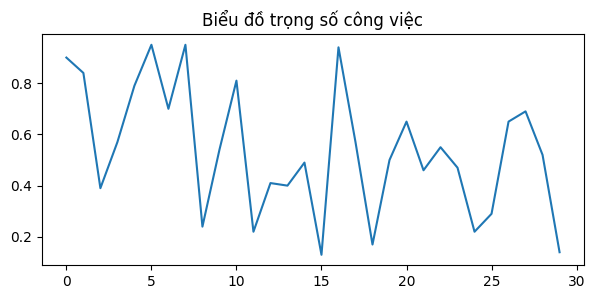
\includegraphics[width=0.7\linewidth]{output_w.png}
\caption{Biểu đồ trọng số công việc.}
\end{figure}

Dựa vào biểu đồ trên, ta có thể thấy rằng sau khi tối ưu hóa danh sách công việc, trọng số của từng công việc có \textbf{xu hướng giảm} từ công việc đầu tiên đến công việc cuối cùng.
\end{frame}

\begin{frame}{Dữ liệu trực quan}

Từ đây, ta dễ dàng nhận thấy rằng các công việc có \textbf{thời gian xử lý ngắn} và \textbf{trọng số (mức độ ưu tiên) cao} sẽ được đẩy lên đầu, trong khi những công việc có thời gian xử lý dài hơn và mức độ ưu tiên thấp hơn sẽ được xếp sau.
\end{frame}

\section{Ứng dụng thực tế}

\section*{Lập kế hoạch gia công thiết kế}

\section*{Giới thiệu về quy trình thiết kế}

\begin{frame}{Giới thiệu về quy trình thiết kế}
\begin{figure}[h]
\centering
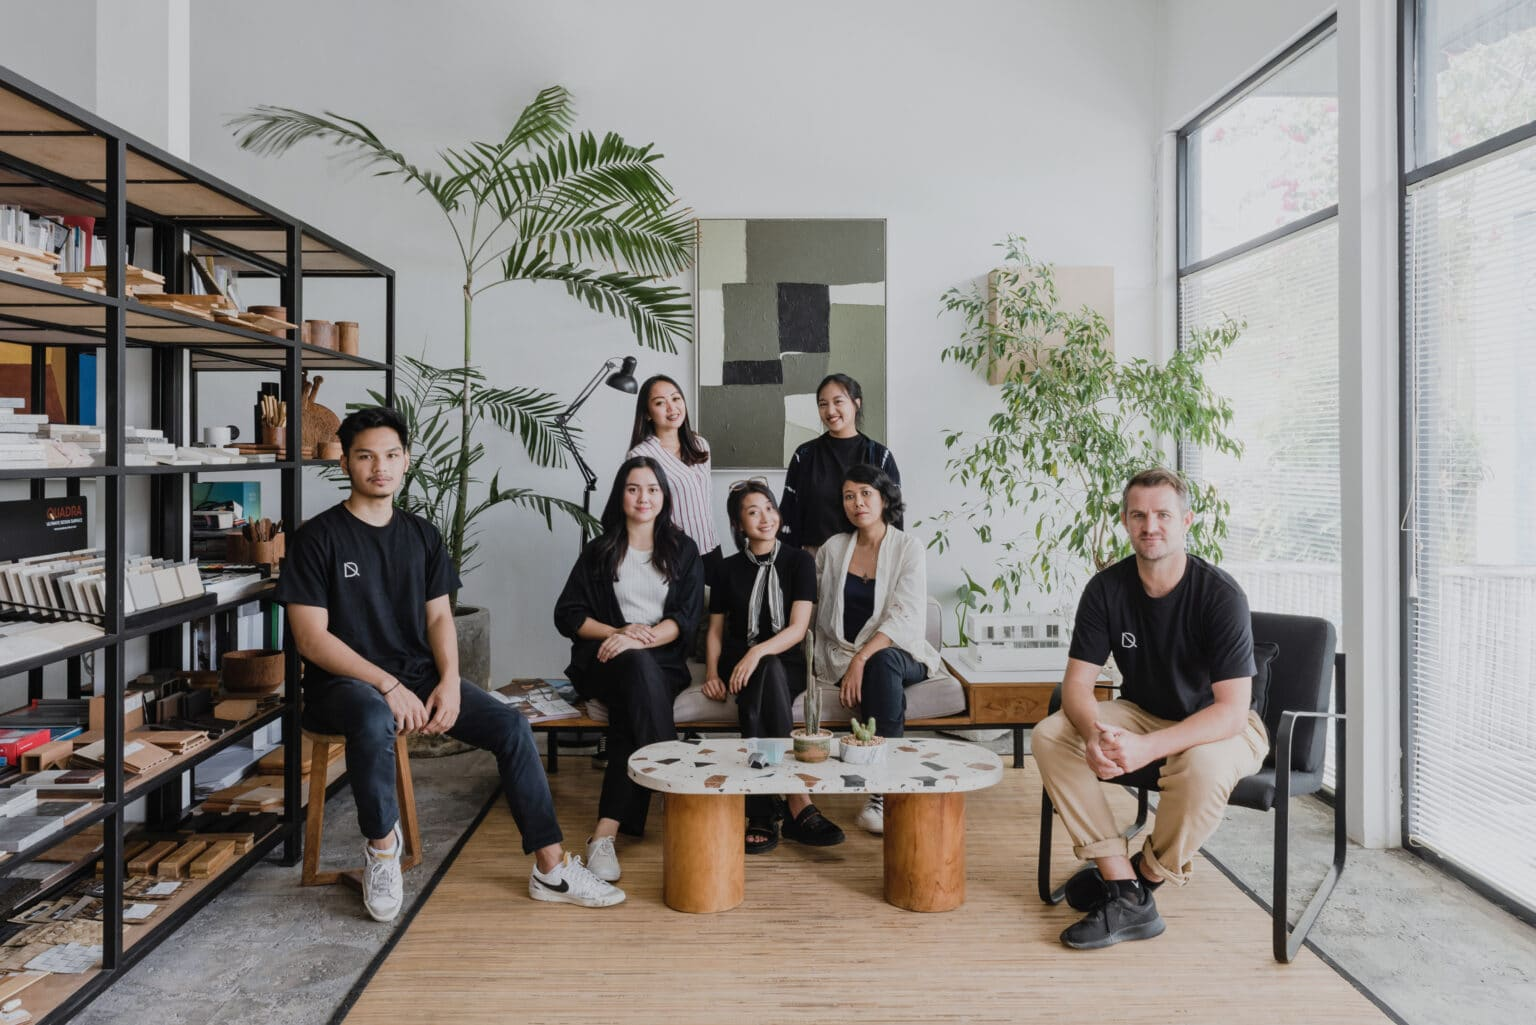
\includegraphics[width=0.5\linewidth]{nt1.jpg}
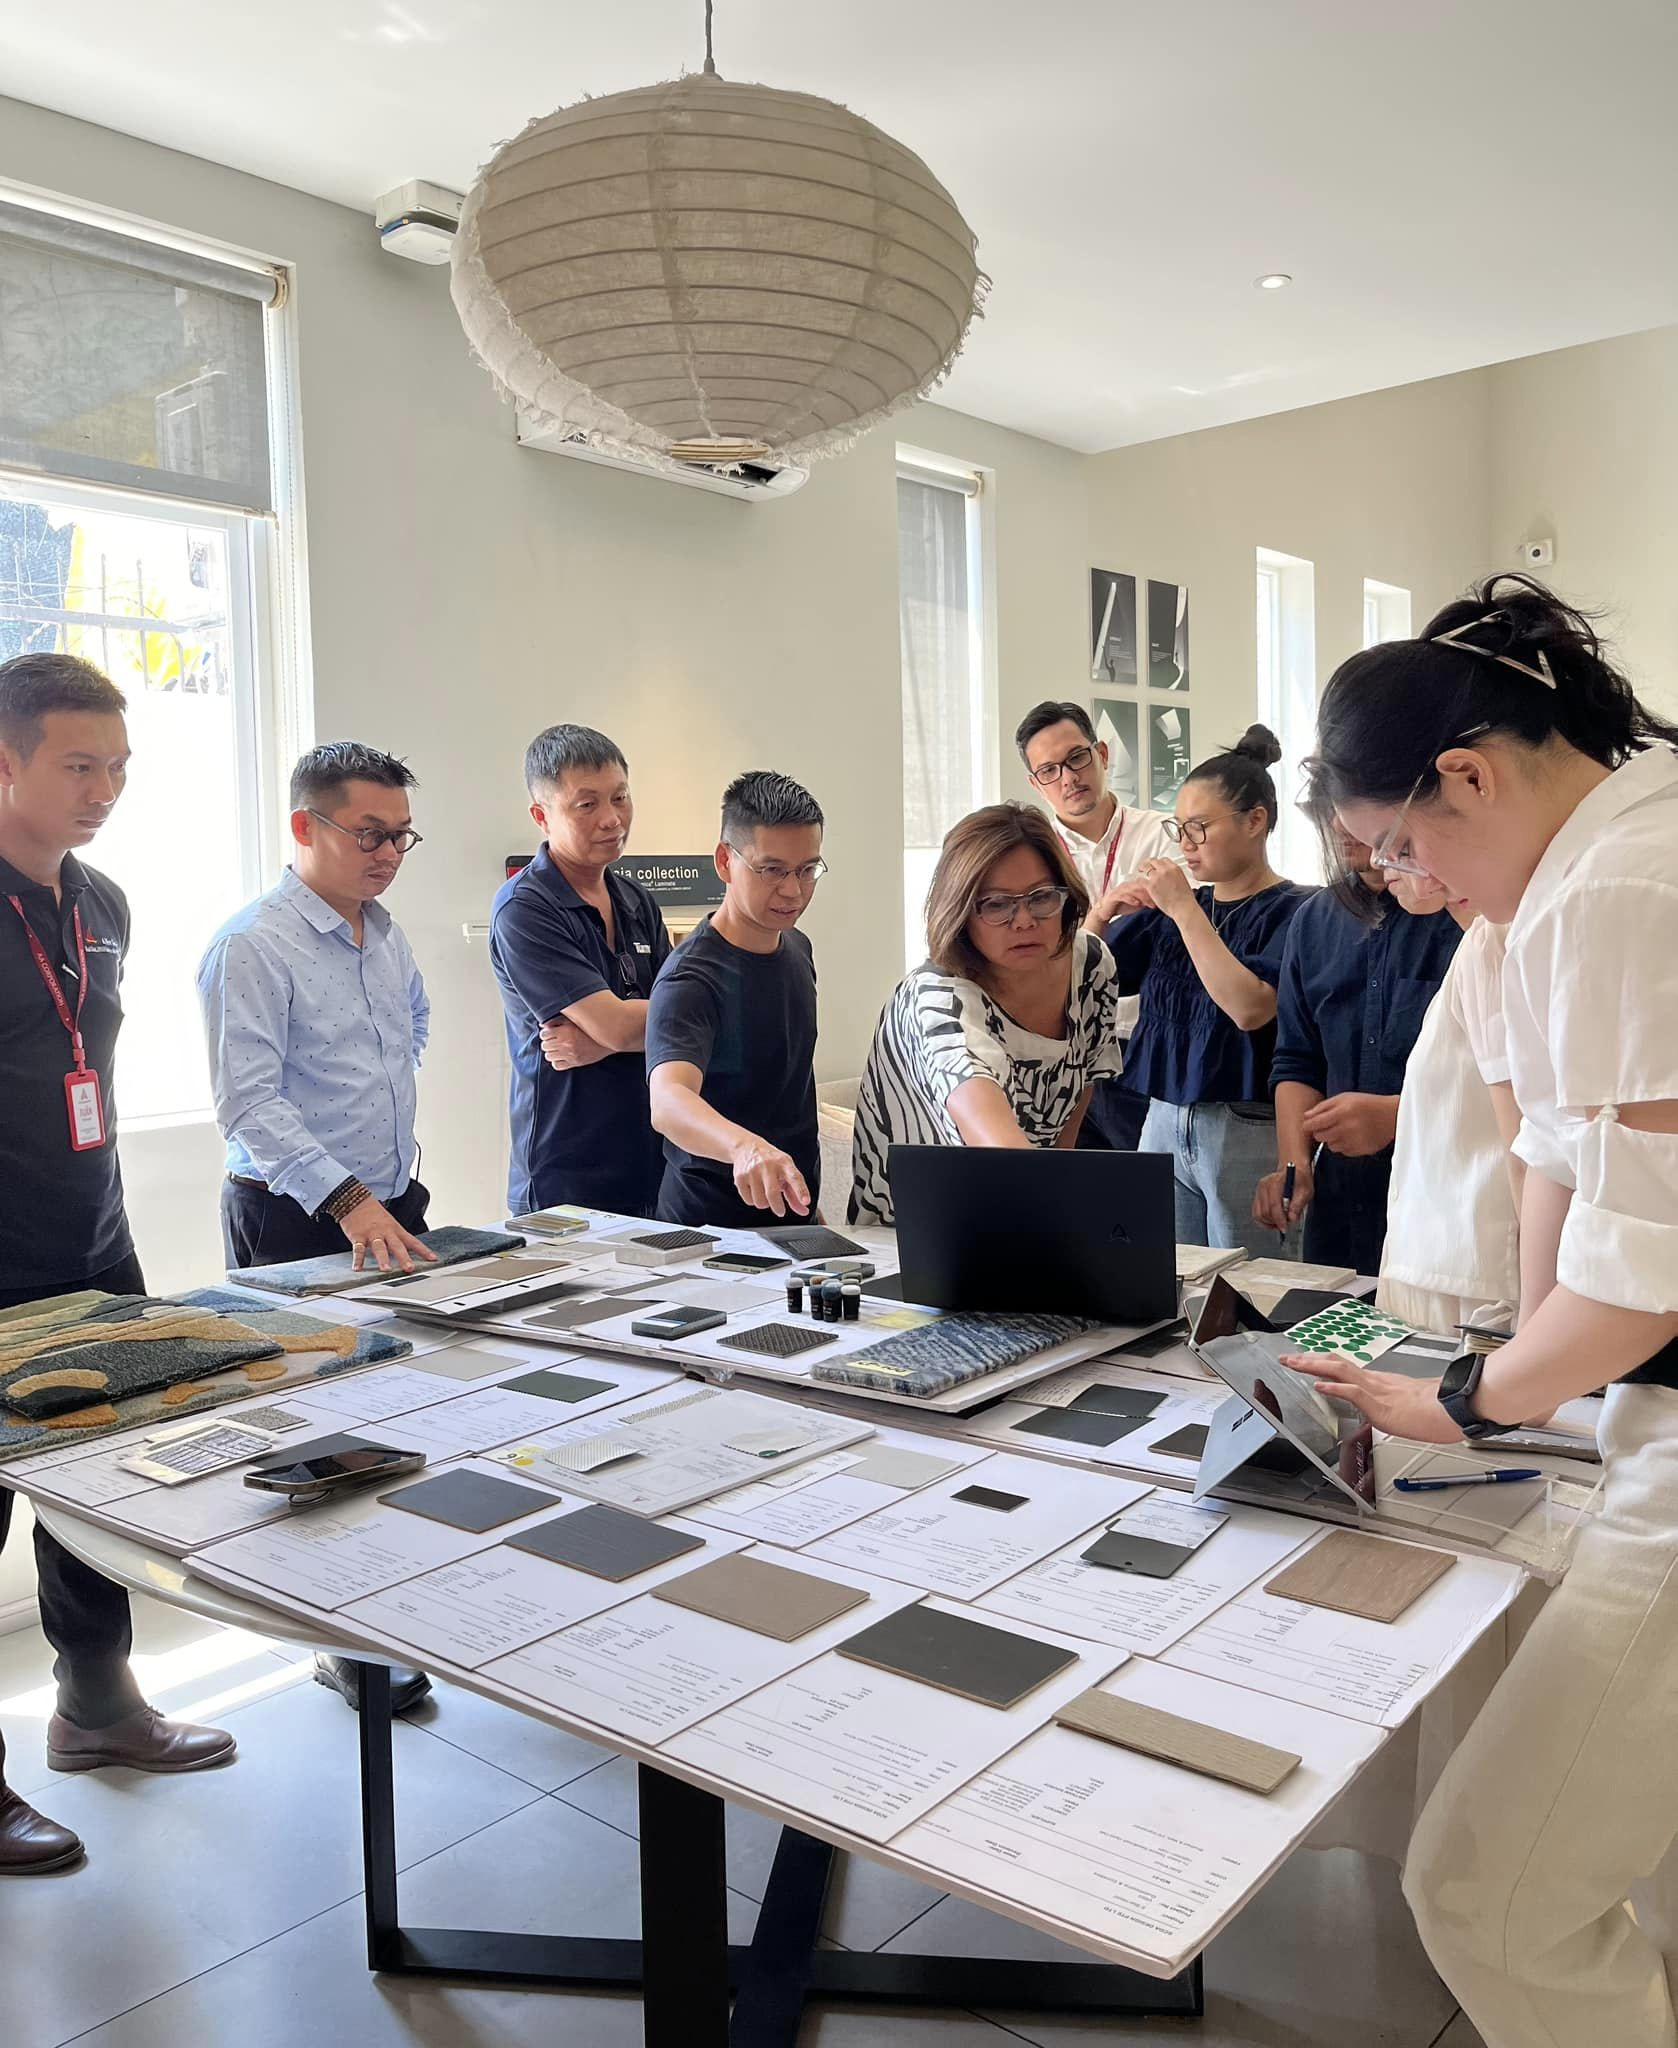
\includegraphics[width=0.274\linewidth]{nt2.jpg}
\end{figure}

\begin{itemize}
\item<1-> Trong quá trình xử lý, studio thường phải đối mặt với việc phân bổ thời gian và quản lý \textbf{nhiều dự án đồng thời}, dựa trên sự ưu tiên, độ phức tạp của từng dự án cũng như thời gian thi công.

\item<2-> Việc áp dụng các \textbf{kỹ thuật lập lịch} giúp quản lý dữ liệu và lập kế hoạch hiệu quả hơn, đồng thời hỗ trợ theo dõi tiến độ và điều chỉnh khi cần thiết.
\end{itemize}
\end{frame}

\begin{frame}{Giới thiệu về quy trình thiết kế}
Thông thường, một dự án thiết kế nội thất sẽ trải qua các giai đoạn chính sau:
\begin{itemize}
\item Phát triển ý tưởng.
\item Quy hoạch không gian.
\item Phát triển thiết kế.
\item Lựa chọn vật liệu.
\item Tính toán chi phí.
\item Xây dựng.
\item Lắp đặt.
\item Decor.
\item Nghiệm thu.
\end{itemize}
\end{frame}

\begin{frame}{Giới thiệu về quy trình thiết kế}
    
\begin{itemize}
\item<1-> Các công đoạn trong một dự án cần được thực hiện theo thứ tự (hay \textbf{ràng buộc thứ tự}). Do đó, bài toán có thể được mô hình hóa dưới dạng bài toán $1|prec|\sum w_j C_j$.

\item<2-> Ngoài ra, studio còn phải thực hiện các công việc khảo sát hiện trạng cho nhiều dự án khác nhau mà không yêu cầu thứ tự thực hiện (hay \textbf{không tồn tại ràng buộc thứ tự}). Trường hợp này có thể được mô hình hóa thành bài toán $1||\sum w_j C_j$.
\end{itemize}
\end{frame}

\begin{frame}{Giới thiệu về quy trình thiết kế}
\begin{vd}

Giả sử studio đang trong giai đoạn thực hiện 3 dự án (công trình) sau:

\begin{itemize} \footnotesize
\item \textbf{SJC Tower} - Dự án A.
\item \textbf{Nguyễn Cư Trinh Centre} - Dự án B.
\item \textbf{Tòa nhà phức hợp Amigo} - Dự án C.
\end{itemize}

Cũng trong quá trình đó, studio cần thực hiện khảo sát hiện trạng cho các công trình sau:
\begin{itemize} \footnotesize
\item \textbf{Tòa nhà văn phòng Fideco} - Khảo sát hiện trạng 1.
\item \textbf{Công trình tại đường Tôn Đức Thắng} - Khảo sát hiện trạng 2.
\item \textbf{Dự án căn hộ và văn phòng tại đường Nguyễn Hữu Cảnh} - Khảo sát hiện trạng 3.
\item \textbf{Dự án cầu đường Nguyễn Khoái} - Khảo sát hiện trạng 4.
\item \textbf{Công trình nhà dân dụng và công nghiệp tại quận 1} - Khảo sát hiện trạng 5.
\item \textbf{IFC One Saigon} - Khảo sát hiện trạng 6.
\item \textbf{One Central Saigon} - Khảo sát hiện trạng 7.
\end{itemize}
\end{vd}
\end{frame}

\section*{Xử lý số liệu bằng TiLearn}

\begin{frame}{Xử lý số liệu bằng TiLearn}
    \begin{table}[ht]
        \centering
        \begin{tabular}{|l|c|c|c|c|}
        \hline
        \textbf{Name} & \textbf{p} & \textbf{r} & \textbf{d} & \textbf{w} \\
        \hline
        Project A - Phát triển ý tưởng    & 4  & 0  & 200 & 0.85 \\
        Project A - Quy hoạch không gian  & 3  & 0  & 200 & 0.80 \\
        Project A - Phát triển thiết kế   & 5  & 0  & 200 & 0.75 \\
        Project A - Lựa chọn vật liệu     & 2  & 0  & 200 & 0.70 \\
        Project A - Tính toán chi phí     & 2  & 0  & 200 & 0.60 \\
        Project A - Xây dựng              & 10 & 0  & 200 & 0.95 \\
        Project A - Lắp đặt               & 4  & 0  & 200 & 0.70 \\
        Project A - Decor                 & 3  & 0  & 200 & 0.85 \\
        Project A - Bàn giao              & 1  & 0  & 200 & 1.00 \\
        \hline
        \end{tabular}
        \caption{Project A - SJC Tower.}
        \end{table}
\end{frame}


\begin{frame}{Xử lý số liệu bằng TiLearn}
    \begin{table}[ht]
        \centering
        \begin{tabular}{|l|c|c|c|c|}
        \hline
        \textbf{Name} & \textbf{p} & \textbf{r} & \textbf{d} & \textbf{w} \\
        \hline
        Project B - Phát triển ý tưởng    & 8  & 0  & 200 & 0.85 \\
        Project B - Quy hoạch không gian  & 7  & 0  & 200 & 0.80 \\
        Project B - Phát triển thiết kế   & 20 & 0  & 200 & 0.95 \\
        Project B - Lựa chọn vật liệu     & 3  & 0  & 200 & 0.70 \\
        Project B - Tính toán chi phí     & 2  & 0  & 200 & 0.60 \\
        Project B - Xây dựng              & 40 & 0  & 200 & 0.95 \\
        Project B - Lắp đặt               & 15 & 0  & 200 & 0.70 \\
        Project B - Decor                 & 9  & 0  & 200 & 0.85 \\
        Project B - Bàn giao              & 1  & 0  & 200 & 1.00 \\
        \hline
        \end{tabular}
        \caption{Project B - Nguyễn Cư Trinh Centre.}
        \end{table}
\end{frame}

\begin{frame}{Xử lý số liệu bằng TiLearn}
    \begin{table}[ht]
        \centering
        \begin{tabular}{|l|c|c|c|c|}
        \hline
        \textbf{Name} & \textbf{p} & \textbf{r} & \textbf{d} & \textbf{w} \\
        \hline
        Project C - Phát triển ý tưởng    & 5  & 0  & 200 & 0.85 \\
        Project C - Quy hoạch không gian  & 2  & 0  & 200 & 0.80 \\
        Project C - Phát triển thiết kế   & 4  & 0  & 200 & 0.75 \\
        Project C - Lựa chọn vật liệu     & 6  & 0  & 200 & 0.70 \\
        Project C - Tính toán chi phí     & 1  & 0  & 200 & 0.60 \\
        Project C - Xây dựng              & 15 & 0  & 200 & 0.95 \\
        Project C - Lắp đặt               & 4  & 0  & 200 & 0.70 \\
        Project C - Decor                 & 4  & 0  & 200 & 0.85 \\
        Project C - Bàn giao              & 1  & 0  & 200 & 1.00 \\
        \hline
        \end{tabular}
        \caption{Project C - Tòa nhà phức hợp Amigo.}
        \end{table}
\end{frame}

\begin{frame}{Xử lý số liệu bằng TiLearn}
    \begin{table}[ht]
        \centering
        \begin{tabular}{|l|c|c|c|c|}
        \hline
        \textbf{Name} & \textbf{p} & \textbf{r} & \textbf{d} & \textbf{w} \\
        \hline
        Khảo sát hiện trạng 1 & 2  & 0  & 200 & 0.33 \\
        Khảo sát hiện trạng 2 & 6  & 0  & 200 & 0.67 \\
        Khảo sát hiện trạng 3 & 5  & 0  & 200 & 0.45 \\
        Khảo sát hiện trạng 4 & 15 & 0  & 200 & 0.85 \\
        Khảo sát hiện trạng 5 & 4  & 0  & 200 & 0.10 \\
        Khảo sát hiện trạng 6 & 4  & 0  & 200 & 0.60 \\
        Khảo sát hiện trạng 7 & 20 & 0  & 200 & 0.70 \\
        \hline
        \end{tabular}
        \caption{Danh sách khảo sát hiện trạng.}
        \end{table}

\end{frame}

\begin{frame}{Xử lý số liệu bằng TiLearn}
Cấu trúc tập tin được thiết lập như sau:
\medskip
\begin{figure}[h]
\centering
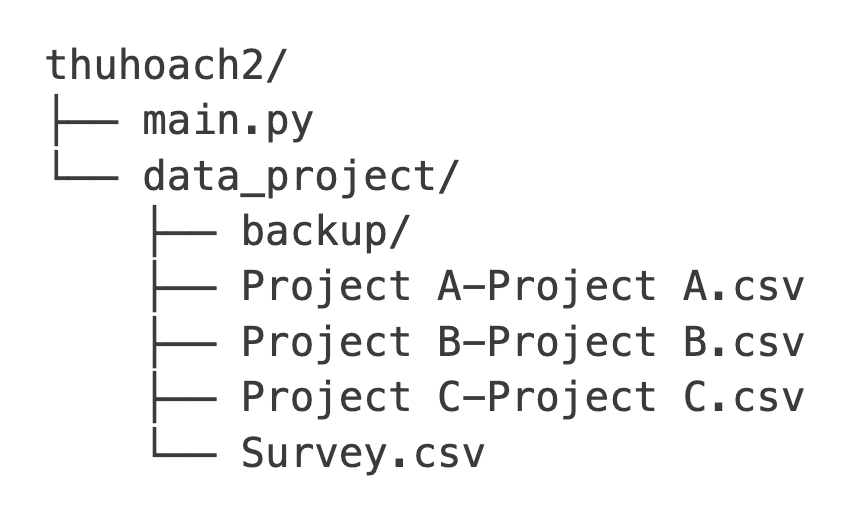
\includegraphics[width=0.6\linewidth]{project_nt.png}
\caption{Cấu trúc tập tin.}
\end{figure}
\end{frame}

\begin{frame}[fragile]{Xử lý số liệu bằng TiLearn}
Ta thực hiện khai báo đường dẫn dữ liệu như sau:
\begin{lstlisting}[language=Python]
    original_project = 'thuhoach2/data_project'
    backup_project = 'thuhoach2/data_project/backup'
    project_A = 'thuhoach2/data_project/Project A-Project A.csv'
    project_B = 'thuhoach2/data_project/Project B-Project B.csv'
    project_C = 'thuhoach2/data_project/Project C-Project C.csv'
    survey = 'thuhoach2/data_project/Survey.csv'
\end{lstlisting}
\end{frame}

\begin{frame}[fragile]{Xử lý số liệu bằng TiLearn}
Tiếp theo, ta chọn dạng bài toán cho từng danh sách bằng cách thiết lập tham số \textbf{prec} như sau:
    
\begin{itemize}
\item \textbf{prec=0} cho bài toán không tồn tại ràng buộc thứ tự.
\item \textbf{prec=1} cho bài toán tồn tại ràng buộc thứ tự.
\end{itemize}

\begin{lstlisting}[language=Python]
    lists_project = [
        pl.List(file_path=project_A, prec=1),
        pl.List(file_path=project_B, prec=1),
        pl.List(file_path=project_C, prec=1),
        pl.List(file_path=survey, prec=0),
    ]
\end{lstlisting}
\end{frame}

\begin{frame}[fragile]{Chạy số liệu minh hoạ}
\onslide<1->{Ta chạy chương trình bằng lệnh sau:}
\begin{lstlisting}[language=Python]
schedule = tl.optimal_list(lists_project,
                            original_project,
                            backup_project)
print(schedule)
\end{lstlisting}

\onslide<2->{{\scriptsize [['Project A - Phát triển ý tưởng', 4.0, 0, 200, 0.85, 0.2125], ['Project A - Quy hoạch không gian', 3.0, 0, 200, 0.8, 0.2357142857142857], ['Project C - Phát triển ý tưởng', 5.0, 0, 200, 0.85, 0.16999999999999998], ['Project C - Quy hoạch không gian', 2.0, 0, 200, 0.8, 0.2357142857142857], ['Project A - Phát triển thiết kế', 5.0, 0, 200, 0.75, 0.15], ['Project A - Lựa chọn vật liệu', 2.0, 0, 200, 0.7, 0.20714285714285713], ['Project A - Tính toán chi phí', 2.0, 0, 200, 0.6, 0.22777777777777775], ['Project A - Xây dựng', 10.0, 0, 200, 0.95, 0.095], ['Project A - Lắp đặt', 4.0, 0, 200, 0.7, 0.11785714285714285], ['Project A - Decor', 3.0, 0, 200, 0.85, 0.14705882352941177], ['Project A - Bàn giao', 1.0, 0, 200, 1.0, 0.19444444444444445], ['Project C - Phát triển thiết kế', 4.0, 0, 200, 0.75, 0.1875], ['Project C - Lựa chọn vật liệu', 6.0, 0, 200, 0.7, 0.11666666666666665], ['Project C - Tính toán chi phí', 1.0, 0, 200, 0.6, 0.1857142857142857], ['Khảo sát hiện trạng 1', 2.0, 0, 200, 0.33, 0.165], ['Khảo sát hiện trạng 6',
}}
    
\end{frame}

\begin{frame}{Chạy số liệu minh hoạ}
\footnotesize
4.0, 0, 200, 0.6, 0.15], ['Project C - Xây dựng', 15.0, 0, 200, 0.95, 0.06333333333333332], ['Project C - Lắp đặt', 4.0, 0, 200, 0.7, 0.08684210526315789], ['Project C - Decor', 4.0, 0, 200, 0.85, 0.10869565217391304], ['Project C - Bàn giao', 1.0, 0, 200, 1.0, 0.14583333333333334], ['Khảo sát hiện trạng 2', 6.0, 0, 200, 0.67, 0.11166666666666668], ['Project B - Phát triển ý tưởng', 8.0, 0, 200, 0.85, 0.10625], ['Project B - Quy hoạch không gian', 7.0, 0, 200, 0.8, 0.11], ['Khảo sát hiện trạng 3', 5.0, 0, 200, 0.45, 0.09], ['Project B - Phát triển thiết kế', 20.0, 0, 200, 0.95, 0.0475], ['Project B - Lựa chọn vật liệu', 3.0, 0, 200, 0.7, 0.07173913043478261], ['Project B - Tính toán chi phí', 2.0, 0, 200, 0.6, 0.09], ['Khảo sát hiện trạng 4', 15.0, 0, 200, 0.85, 0.056666666666666664], ['Project B - Xây dựng', 40.0, 0, 200, 0.95, 0.02375], ['Project B - Lắp đặt', 15.0, 0, 200, 0.7, 0.03], ['Project B - Decor', 9.0, 0, 200, 0.85, 0.0390625], ['Project B - Bàn giao', 1.0, 0, 200, 1.0, 0.05384615384615385], ['Khảo sát hiện trạng 7', 20.0, 0, 200, 0.7, 0.034999999999999996], ['Khảo sát hiện trạng 5', 4.0, 0, 200, 0.1, 0.025]]
\end{frame}

\section*{Dữ liệu trực quan}

\begin{frame}{Dữ liệu trực quan}
\begin{figure}[h]
\centering
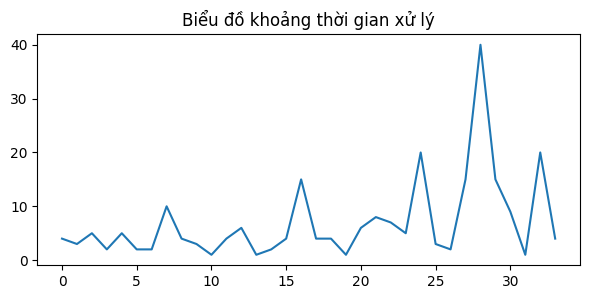
\includegraphics[width=0.7\linewidth]{output_project_p.png}
\caption{Biểu đồ khoảng thời gian xử lý.}
\end{figure}

Dựa vào biểu đồ trên, có thể thấy rằng sau khi tối ưu hóa danh sách công việc, thời gian xử lý của từng công việc có \textbf{xu hướng tăng} từ công việc đầu tiên đến công việc cuối cùng.
\end{frame}

\begin{frame}{Dữ liệu trực quan}
\begin{figure}[h]
\centering
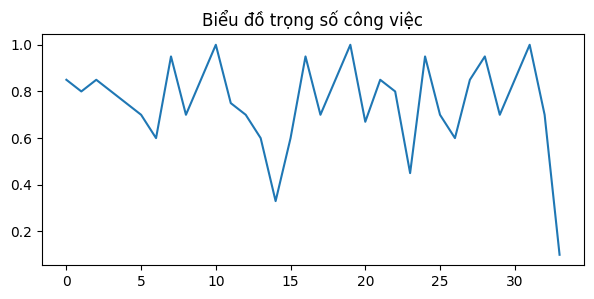
\includegraphics[width=0.7\linewidth]{output_project_w.png}
\caption{Biểu đồ trọng số công việc.}
\end{figure}

Dựa vào biểu đồ trên, ta có thể thấy rằng sau khi tối ưu hóa danh sách công việc, trọng số của từng công việc có \textbf{xu hướng giảm} từ công việc đầu tiên đến công việc cuối cùng.
\end{frame}

\begin{frame}{Dữ liệu trực quan}

Từ đây, ta dễ dàng nhận thấy rằng các công việc có \textbf{thời gian xử lý ngắn} và \textbf{trọng số (mức độ ưu tiên) cao} sẽ được đẩy lên đầu, trong khi những công việc có thời gian xử lý dài hơn và mức độ ưu tiên thấp hơn sẽ được xếp sau.

Từ đó giúp tối ưu hoá quy trình dự án một cách hiệu quả.
\end{frame}



\begin{frame}[allowframebreaks, noframenumbering]
    \nocite{*}
    \printbibliography
\end{frame}


\begin{frame}
    \begin{block}{}
    \medskip
    \center{\huge \it \textcolor[rgb]{0.37, 0.150, 0.190}{Thanks for listening!}}
    \medskip
    \end{block}	
\end{frame}    
\end{document}
